\chapter{Emisi\'on de radio de una EAS}
\label{ch:easRadio}

En este capítulo se abordará la emisión de radio de las lluvias atmosféricas extendidas.
Se discutirán sus características y sus mecanismos de emisión así como un modelo simplificado que permite, mediante razonamientos elementales recuperar sus características principales.

\section{Mecanismos de emisi\'on}
	\label{sc:emision}
	
	Con el fin de explotar todo el potencial de un detector de antenas de radio, conocer el proceso de emisión es fundamental. 
	Este es un fenómeno complicado en el que influyen una gran cantidad factores, como por ejemplo, la distribuciones longitudinal y transversal de partículas y energía de la EAS, el campo geomagnético, etc.
	Sin embargo, puede ser entendido mediante dos mecanismos efectivos llamados el efecto geomagn\'etico y el efecto Askaryan.
	
	\subsection{Efecto geomagn\'etico}
	
	Este se refiere a la interacción entre las partículas cargadas y el campo magn\'etico terrestre.
	Durante la evoluci\'on de la EAS, debido a la fuerza de Lorentz los \el{+} y \el{-} se deflectan en direcciones opuestas, lo que produce una corriente efectiva, como se esquematiza en el panel izquierdo de la figura \ref{fig:geom_sketch}.
	Dicha corriente, dado que es generada proporcionalmente a $-\vec\beta\times \vec B$, es practicamente perpendicular tanto al eje de la lluvia como al campo magn\'etico terrestre.
	En consecuencia el campo el\'ectrico generado posee una polarizaci\'on uniforme sobre la superficie de la tierra, lo que se observa en el panel derecho de la figura \ref{fig:geom_sketch}.
	Por otra parte, debido a que la magnitud de la corriente efectiva depende fuertemente de la velocidad de drift de los \el{+} y \el{-}, que a su vez depende directamente de la densidad de la atm\'osfera, no es sorprendente que este sea el mecanismo predominante cuando la lluvia se inicia a gran altitud.
	
	\begin{figure}[ht!]
		\centering
		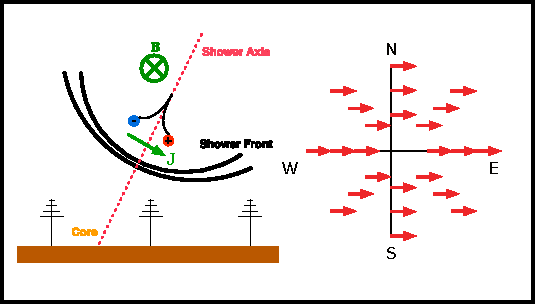
\includegraphics[width=0.75\textwidth]{fig/EASRadio/geom_sketch}
		\caption{\label{fig:geom_sketch} Izquierda: representaci\'on del efecto geomagnético.
		Derecha: polarización del campo eléctrico generado por el efecto geomagnético a nivel del suelo.}
	\end{figure}
	
	\subsection{Efecto Askaryan}
	
	El segundo mecanismo de emisión relevante fue estudiado por Askaryan en 1962 \cite{askaryan1962} y se basa en que tanto el efecto compton como la generacion de rayos delta provocan un exceso de carga negativa durante el desarrollo de la lluvia, lo que puede considerarse como el movimiento de una carga efectiva.
	Este exceso a su vez es favorecido por la aniquilaci\'on de los positrones con los electrones de los \'atomos atmosf\'ericos. 
	El panel izquierdo de la figura \ref{fig:ask_sketch} muestra un esquema del efecto Askaryan.
	
	Esta carga efectiva genera un campo proporcional a $-\left[\hat u \times \hat u \times \vec\beta\right]$, donde $\hat u$ es la direcci\'on entre la carga que se desplaza y el observador.
	Por ende, el campo eléctrico producido se encuentra polarizado en dirección radial respecto del punto de impacto del eje de la lluvia, tal como se esquematiza en el panel derecho de la figura \ref{fig:ask_sketch}.
	
	\begin{figure}[ht!]
		\centering
		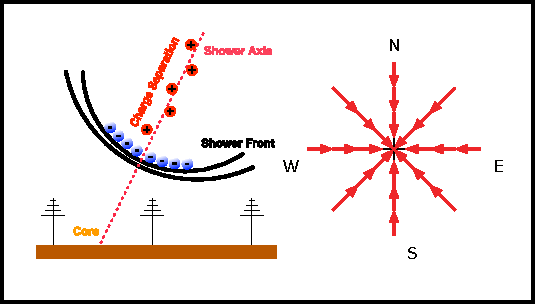
\includegraphics[width=0.75\textwidth]{fig/EASRadio/ask_sketch}
		\caption{\label{fig:ask_sketch} Izquierda: representaci\'on del efecto Askaryan.
		Derecha: polarización del campo eléctrico generado por el efecto Askaryan a nivel del suelo.}
	\end{figure}
	
	
	\subsection{Geometr\'ia de la emisi\'on}
	\label{sbsc:geom_emision}
	
	Las características principales de la emisión pueden entenderse como una superposición de estos efectos, que dependen fuertemente de la evolución de la lluvia y, en particular, de la de su cantidad de partículas.
	Esta superposición provoca que la intensidad de campo electrico tenga una fuerte dependencia en el tiempo y la posición del observador.
	Es por esto que resulta razonable abordar este cálculo mediante simulaciones de Monte Carlo, lo que se tratará en el capítulo \ref{ch:simulacionRadio}.
	
	Un aspecto importante respecto a la geometría de la emisión se produce debido a que las cargas y corrientes inducidas por los efectos Askaryan y geomagn\'etico se desplazan a una velocidad mayor a la de la luz en la atm\'osfera ($n\sim1.0003$), provocando efecto \cher{}.
	La ecuación \ref{eq:chAngle} muestra una estimación del valor de su \'angulo.
	\begin{equation}
	\cos\theta_{ch} = \frac{1}{n} \sim \frac{1}{1.0003}
	\,\, \Rightarrow \,\,
	\theta_{ch} \sim 1.4^\circ
	\label{eq:chAngle}
	\end{equation}
	Como es posible observar, la emisi\'on de radio de las EAS es esencialmente en la direcci\'on de la lluvia.
	
	Existen otras dos resultados interesantes respecto de la geometría de la señal al nivel del suelo que se desprenden de la dependencia de los efectos Askaryan y geomagnético con la densidad de partículas.
	El primero consiste en que la mayor amplitud de la señal se espera en el anillo formado por la intersección entre el cono \cher{} que se proyecta desde el máximo de la lluvia y el suelo, que muestra la figura \ref{fig:cono}.
	
	\begin{figure}[ht!]
		\centering
		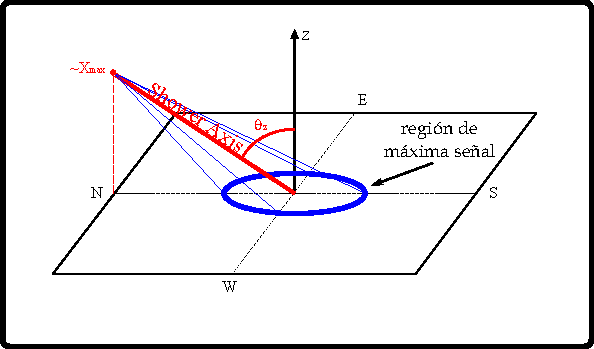
\includegraphics[width=0.7\textwidth]{fig/EASRadio/chConeSch}
		\caption{\label{fig:cono} La región de máxima señal a nivel del suelo se encuentra en la intersección entre el cono \cher{} que se proyecta desde el máximo de la lluvia y el suelo.}
	\end{figure}
	
	El segundo reside en que la coherencia de la señal se mantiene hasta frecuencias más altas en esa región.
	En la figura \ref{fig:chConeSig} se muestra la amplitud de la señal a diferentes frecuencias como función de la coordenada Este-Oeste de la lluvia, obtenida a partir de simulaciones.
	\begin{figure}[ht!]
	\centering
		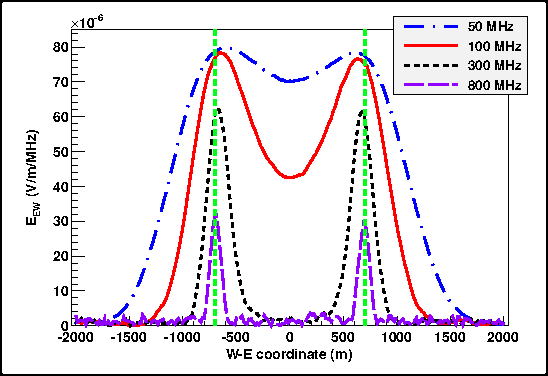
\includegraphics[width=0.7\textwidth]{fig/EASRadio/chConeSig}
		\caption{\label{fig:chConeSig} Amplitud del espectro de se\~nal como funci\'on de la coordenada Este-Oeste de a lluvia obtenido a partir de simulaciones. En l\'inea punteada verde se grafica la posici\'on de impacto del cono \cher{}}
	\end{figure}
	En lineas verdes, y en coincidencia con los máximos para todas las frecuencias se resalta el anillo \cher{} en esa coordenada.
	Se observa que a medida que la frecuencia filtrada aumenta la coherencia se mantiene sólo cerca de dicho anillo.
	
	Ambos resultados pueden comprenderse tambi\'en si se tiene en cuenta que la señal en un observador es la contribución de la señal generada por cada partícula de la lluvia, sin necesidad de recurrir.
	En primer lugar 
	
	
	\subsubsection{Geometr\'ia de la emisi\'on en eventos ES}
	
	Como ya se ha remarcado en el capítulo \ref{ch:easAuger}, las lluvias ES son fundamentalmente diferentes de las lluvias verticales y en cuanto a la emisión de radio no hay excepción. 
	Como se grafica en la figura \ref{fig:chConeES}, la proyección del cono \cher{} sobre el suelo no es una elipse sino una hipérbola.
	\begin{figure}[ht!]
	\centering
		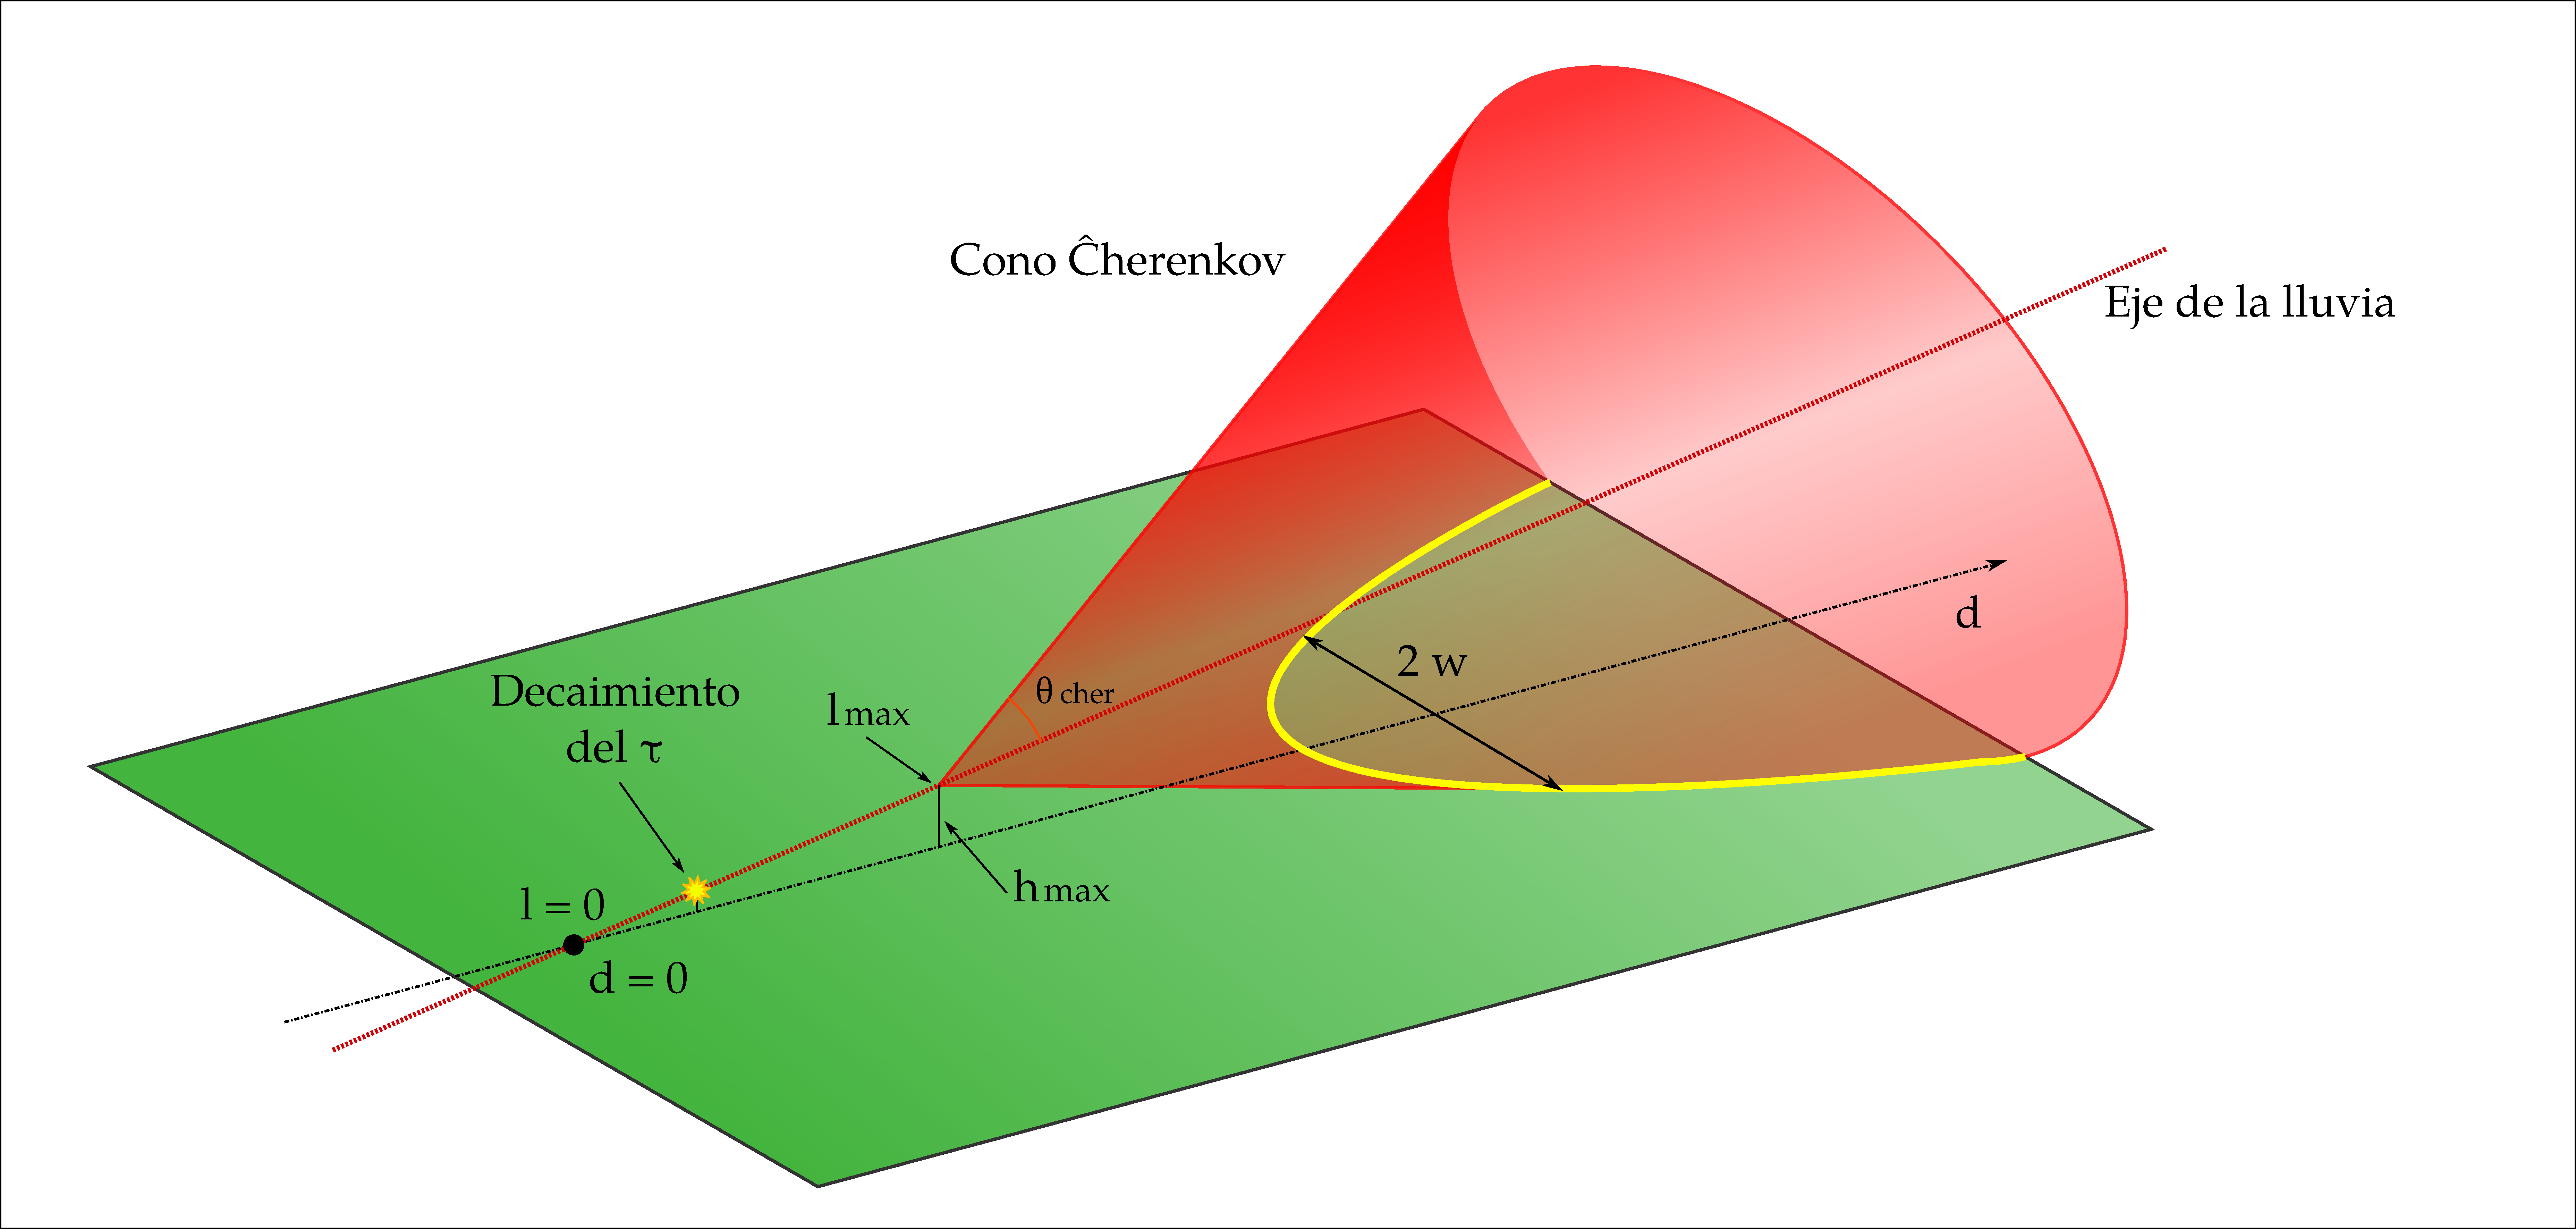
\includegraphics[width=0.85\textwidth]{fig/EASRadio/coneProy}
		\caption{\label{fig:chConeES} La proyección del cono en el suelo para una lluvia ES es ua hiperbola.}
	\end{figure}
	La ecuación \ref{eq:conewidth} muestra la expresión con la que se calcula el ancho $w$ de dicha hiperbola como función de la coordenada $d$.
	\begin{equation}
	w^2=
	(\tan^2 \theta_{cher}-\tan^2 (\theta-\frac{\pi}{2}))
	(\frac{d}{\sin \theta}-l_{max})^2
	- \tan (\theta-\frac{\pi}{2}) \frac{h_{max}}{\sin \theta} (\frac{d}{\sin \theta}-l_{max})
	- \frac{h_{max}^2}{\sin^2 \theta}
	\label{eq:conewidth}
	\end{equation}
	Entran como parámetros el ángulo \cher{} $\theta_{cher}$, el ángulo zenital de la lluvia $\theta$ y la posición del máximo de la lluvia $h_{max}$ y $l_{max}$.
	Los detalles de este cálculo pueden encontrarse en el apendice \ref{ap:intPlanCon}.
	
	La figura \ref{fig:chConeWidth} muestra el ancho en función de $d$ para $l_{max}=10000 \rm m$ y $h_{max}=l_{max}\cos \theta \rm m$.
	\begin{figure}[ht!]
	\centering
		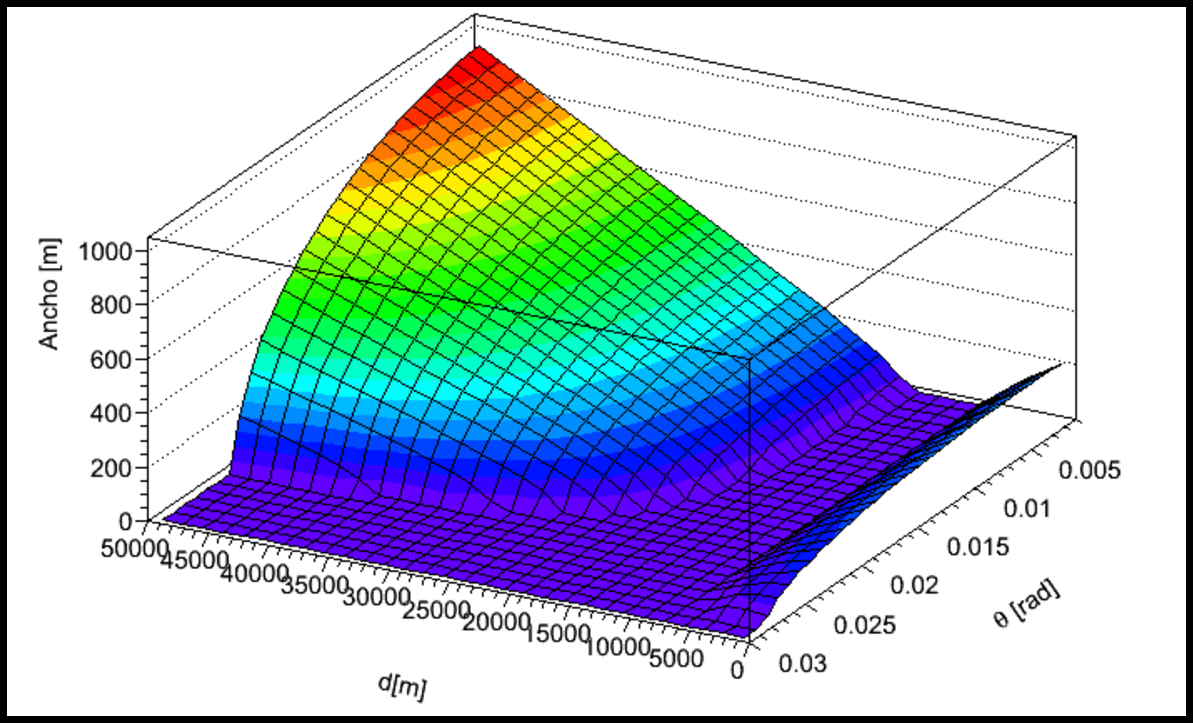
\includegraphics[width=0.85\textwidth]{fig/EASRadio/anchoLluvia}
		\caption{\label{fig:chConeWidth} Ancho del cono \cher{} como función de $d$ y $\theta$ para $l_{max}=10000 \rm m$ y $h_{max}=l_{max}\cos \theta \rm m$. Los valores del ancho por debajo de \cant{d=10000}{m} corresponden a una solición espúrea de la ecuación \ref{eq:conewidth}.}
	\end{figure}
	La primer observación a esta figura es que la emisión es realmente hacia adelante, ya que el ancho es del orden de los \cant{1000}{m} para un $d$ en el orden de los $\rm km$.
	Este aspecto será fundamental a la hora de separar este tipo de lluvias del fondo de lluvias iniciadas por protones o núcleos alto en la atmósfera.
	La segunda observación es que existe un ángulo de corte $\theta_{cut}=90^\circ+\theta_{cher}$ a partir del cuál el cono \cher{} calculado teóricamente no impacta contra el suelo (la ecuación \ref{eq:conewidth} no tiene solución real si el término $\tan^2 \theta_{cher}-\tan^2 (\theta-\frac{\pi}{2})$ es negativo).
	De aquí se desprende que el máximo ángulo zenithal con el que se un detector de superficie podría tener trigger será del orden de $92^\circ$, algunos grados menos que Auger ($\sim95^\circ$).
	
\section{Señal generada por neutrinos ES - Modelo de juguete}

	El objetivo de esta parte de la tesis es estimar las capacidades y limitaciones que presentaría un arreglo de antenas de radio al detectar neutrinos ES.
	Es por esto aquí se desarrolla un modelo unidimensional de juguete, siguiendo la filosofía utilizada en el trabajo de Alvarez-Muñiz \cite{zhairezAir}, y que a partir de suposiciones simples permite recuperar varias características importantes de la señal generada a nivel del suelo.
	
	Supongamos que de la tierra emerge un $\tau$ con ángulo zenital $\theta$ y decae a una altura $h_d$, como se esquematiza en la figura \ref{fig:esRadio_schema}. 
	\begin{figure}[ht!]
		\centering
		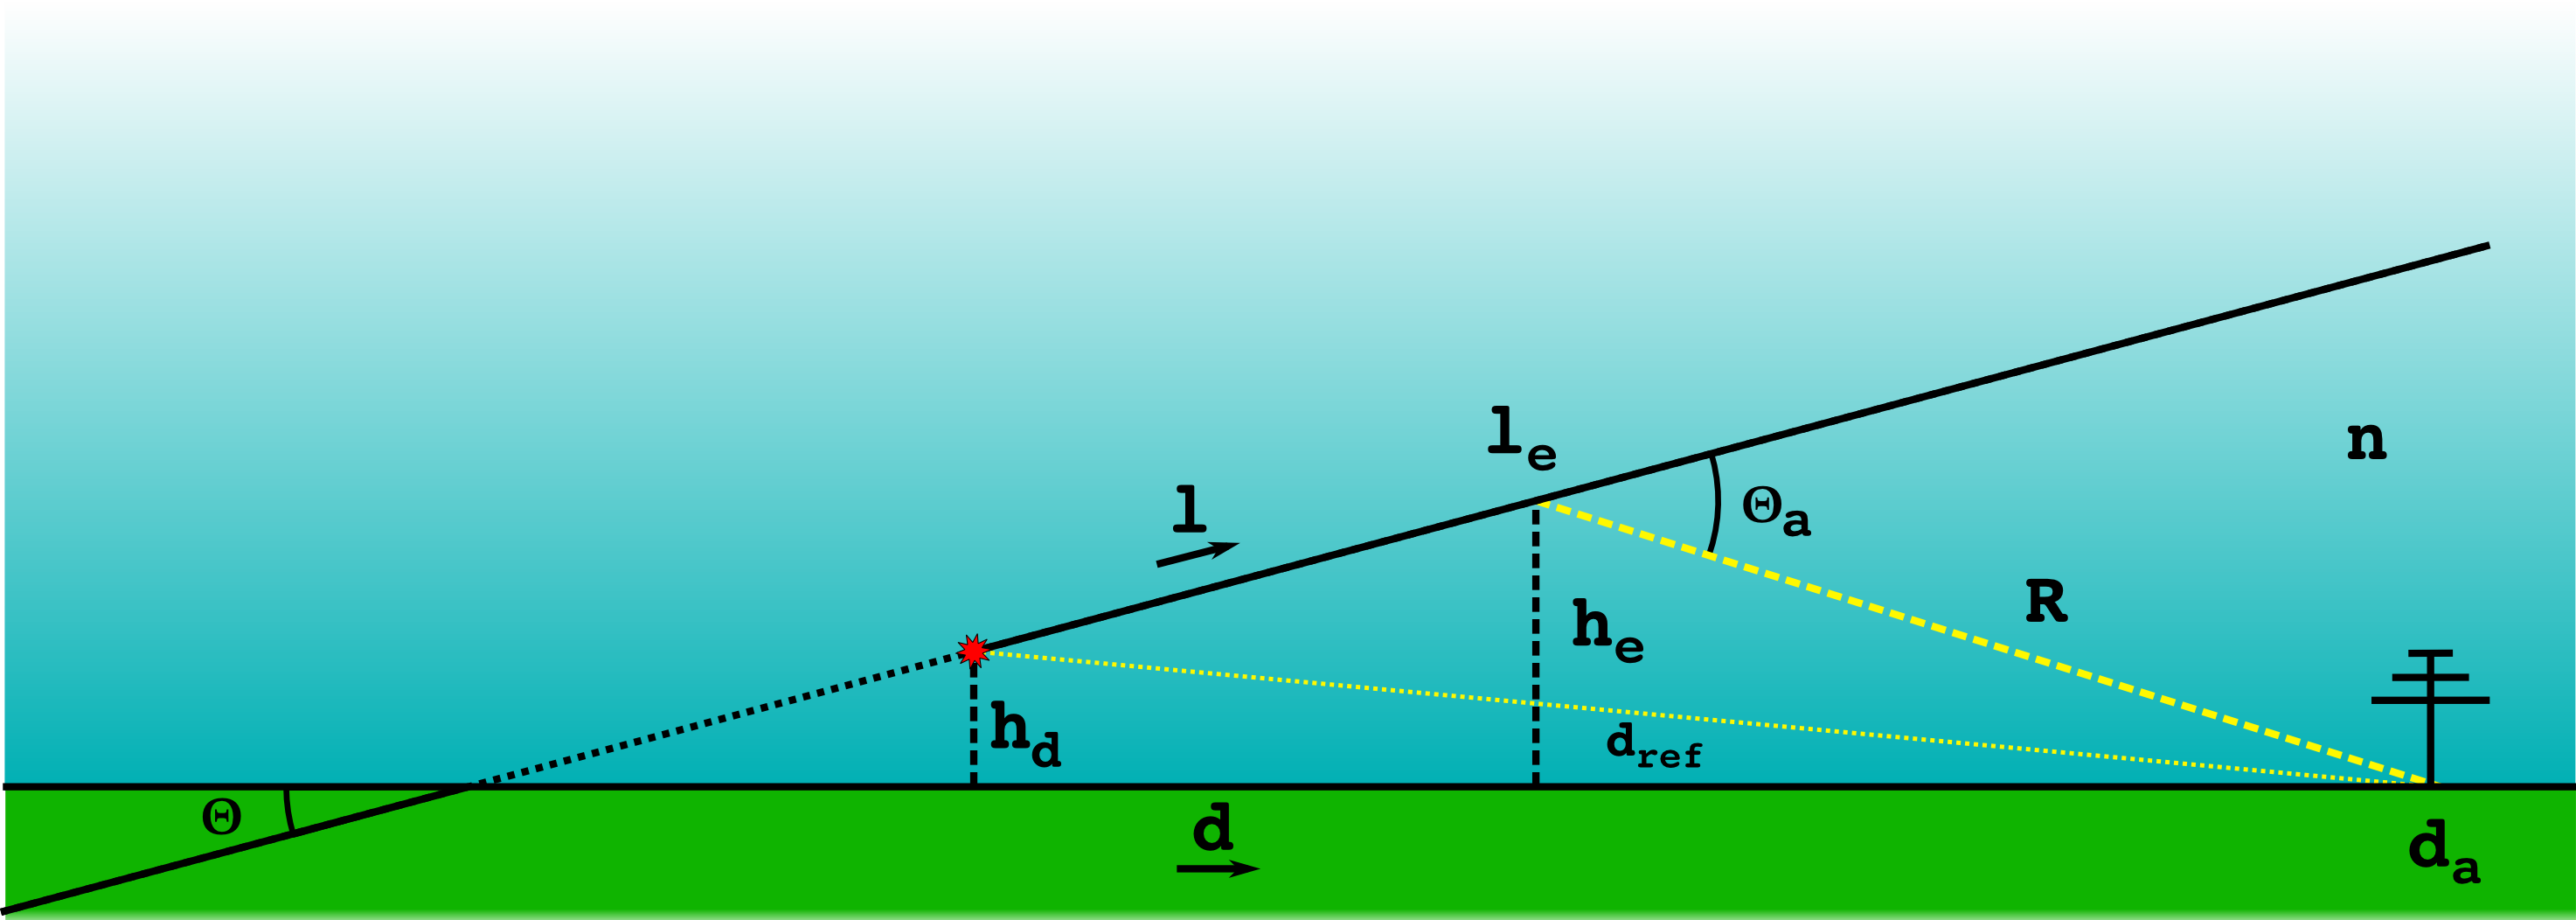
\includegraphics[width=0.95\textwidth]{./fig/EASRadio/timeDelaySchema}
		\caption{\label{fig:esRadio_schema}
		Esquema 
		}
	\end{figure}
	En esta se señalan las coordenadas $d$ y $l$ correspondientes a la distancia sobre el suelo y el eje de la lluvia respectivamente, y medidas desde el punto de decaimiento.
	
	Nuestro objetivo es calcular la señal en una antena ubicada en una posición $d_a$ arbitraria.
	Para ello consideraremos la señal proveniente de cada punto de emisión $l_e$ de la lluvia, la distancia $R$ entre el punto de emisión y la antena, y la distancia de referencia $d_{ref}$ correspondiente a la que tiene que recorrer la señal emitida en el punto de decaimiento.
	Con todo esto, las hipótesis del modelo son las siguientes:
	\begin{enumerate}
	 \item El frente de la lluvia es la única parte de la misma que emite y se desplaza a la velocidad de la luz.
	 \item El tiempo de llegada de la señal emitida desde $l_e$ a la antena se calcula como la suma del tiempo de llegada del frente hasta $l_e$ el tiempo que le toma recorrer al pulso desde $l_e$ hasta la antena.
	 \item Si las señales correspondientes a dos puntos de emisión llegan al mismo tiempo\footnote{En el mismo bin temporal} a la antena, se suman.
	 \item La señal emitida desde $l_e$ tiene un peso correspondiente al producto entre una Gaiser-Hillas en ese punto y el factor $1/R$, donde $R$ es la distancia entre el punto de emisión y la antena.
	\end{enumerate}
	
	Utilizando 1 y 2, el retardo de la señal como función del ángulo de la lluvia, de la altura de decaimiento del $\tau$, de la posición del observador y del punto de emisión se muestra en la ecuación \ref{eq:toytimedelay1}.
	\begin{equation}
	\begin{array}{rcl}
	t & = & \frac{1}{c}\left(l_e+nR(d_a,l_e,h_d,\theta)-nd_{ref}(d_a,l_e,h_d,\theta)\right)
	\end{array}
	\label{eq:toytimedelay1}
	\end{equation}
	En esta se distinguen las tres contribuciones expuestas en el punto 2, el tiempo que tarda el frente en llegar a $l_e$, el tiempo que le toma la señal llegar desde el punto de emisión a la antena a través de un medio de índice de refracción $n$ y se resta el tiempo de referencia que le toma a la señal recorrer $d_{ref}$.
	Luego, utilizando trigonometría básica se consigue la expresión de la ecuación \ref{eq:toytimedelay2}.
	\begin{equation}
	\begin{array}{rcl}
	t & =  & 
	 \frac{1}{c}\left[l_e +
		n \sqrt{h_d^2+d_a^2+l_e^2+2h_dl_e \sin\theta - 2d_al_e\cos\theta} 
		-
		n \sqrt{h_d^2+d_a^2}
		\right]
	\end{array}
	\label{eq:toytimedelay2}
	\end{equation}
	
	A partir de aquí, eliminaremos dos de los cuatro parámetros fijando $\theta=90.5^\circ$ y $h_d=50 \rm m$.
	En la figura \ref{fig:timeDelay_at} se grafica $t(l)$ en estas condiciones para diferentes valores de $d_a$.
	\begin{figure}[ht!]
		\centering
		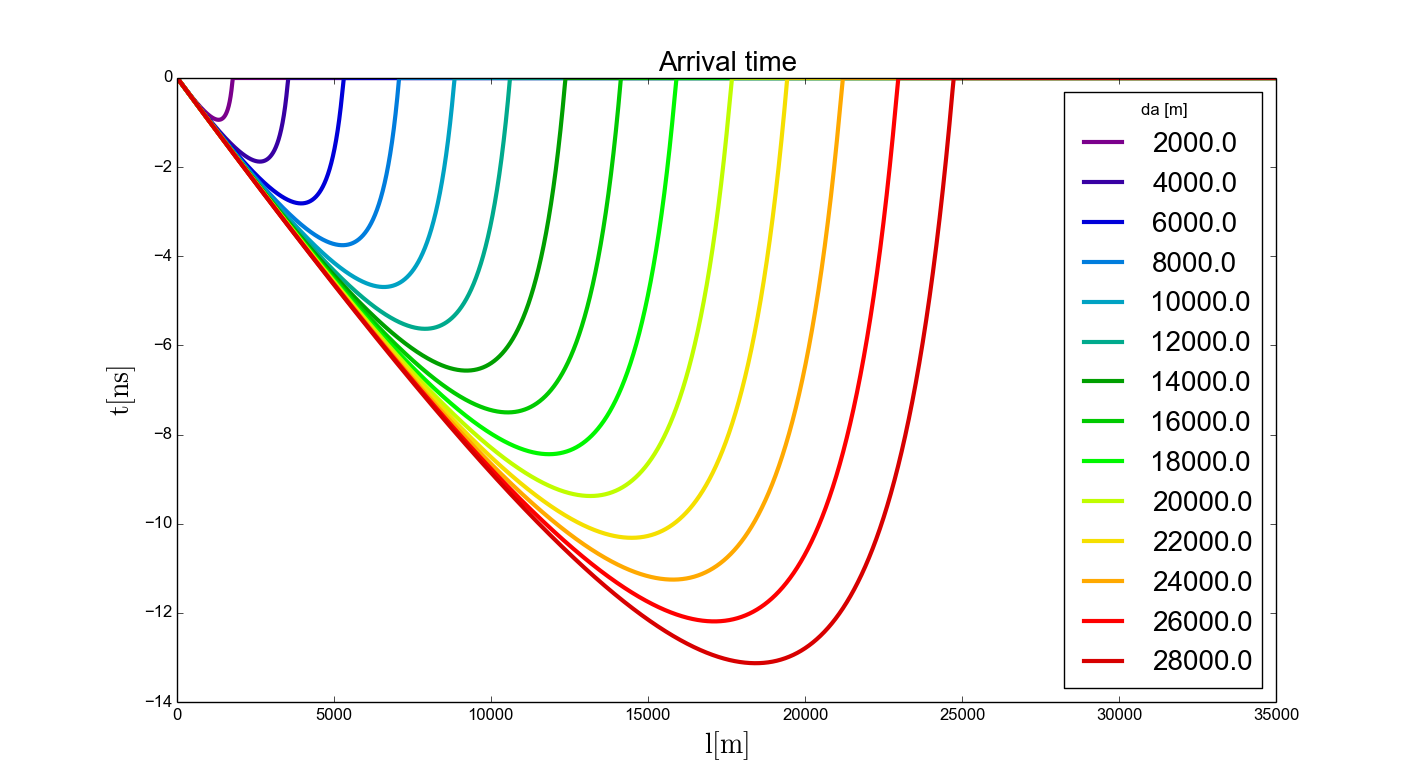
\includegraphics[width=0.8\textwidth]{./fig/EASRadio/timeDelay_at}
		\caption{\label{fig:timeDelay_at}
		Tiempo de arrivo respecto de $d_{ref}/c$ como funci\'on del punto de emisi\'on a lo largo del eje de la lluvia. Los distintos colores representan antenas a diferentes distancias del punto de decaimiento del \tauon{} 
		}
	\end{figure}
	Para una cierta posición de la antena, el tiempo de arrivo a $l=0$ es exactamente el de referencia, por ello todas las curvas comienzan en $t = 0$.
	La pendiente negativa al comienzo se debe a que si bien el trayecto que hay que considerar es mayor que la distancia de referencia ($l_e+R>d_{ref}$ en la figura \ref{fig:esRadio_schema}), la primer parte del recorrido lo realiza la lluvia a velocidad $c$ y la segunda la señal a $c/n$,  por consiguiente, el tiempo de arrivo obtenido es negativo ($t<0$).
	Este efecto llega a un máximo para cierto valor de $l$, generando un tiempo de arrivo mínimo, y luego disminuye para valores de $l$ grandes, como muestra la curva de pendiente positiva.
	
	Como indica el punto 3 del modelo, si la señal proveniente de dos lugares de la lluvia llegan a cierta antena al mismo tiempo estas se suman, por lo que los bines con mayor señal serán tales que $dt/dl\sim0$.
	
	Por otro lado, tambien será necesario considerar el peso asignado por el modelo al punto $l_e$, que como se indica en el punto 4. 
	Dado que tanto el efecto Askaryan y como el geomagnético son proporcionales a la densidad de partículas es razonable pesar utilizano una función de Gaiser-Hillas.
	Por otro lado, hay que tener en cuenta el decaimiento del término de radiación que va como $1/R$.
	En la figura \ref{fig:timeDelay_pd} se muestra en línea punteada la distribución de Gaiser-Hillas para una lluvia cuyo máximo se encuentra a los \cant{10000}{m} del inicio (\cant{\sim10^{18}}{eV}), mientras que en línea llena se grafica el término $1/R$ para diferentes valores de $d_a$.
	\begin{figure}[ht!]
		\centering
		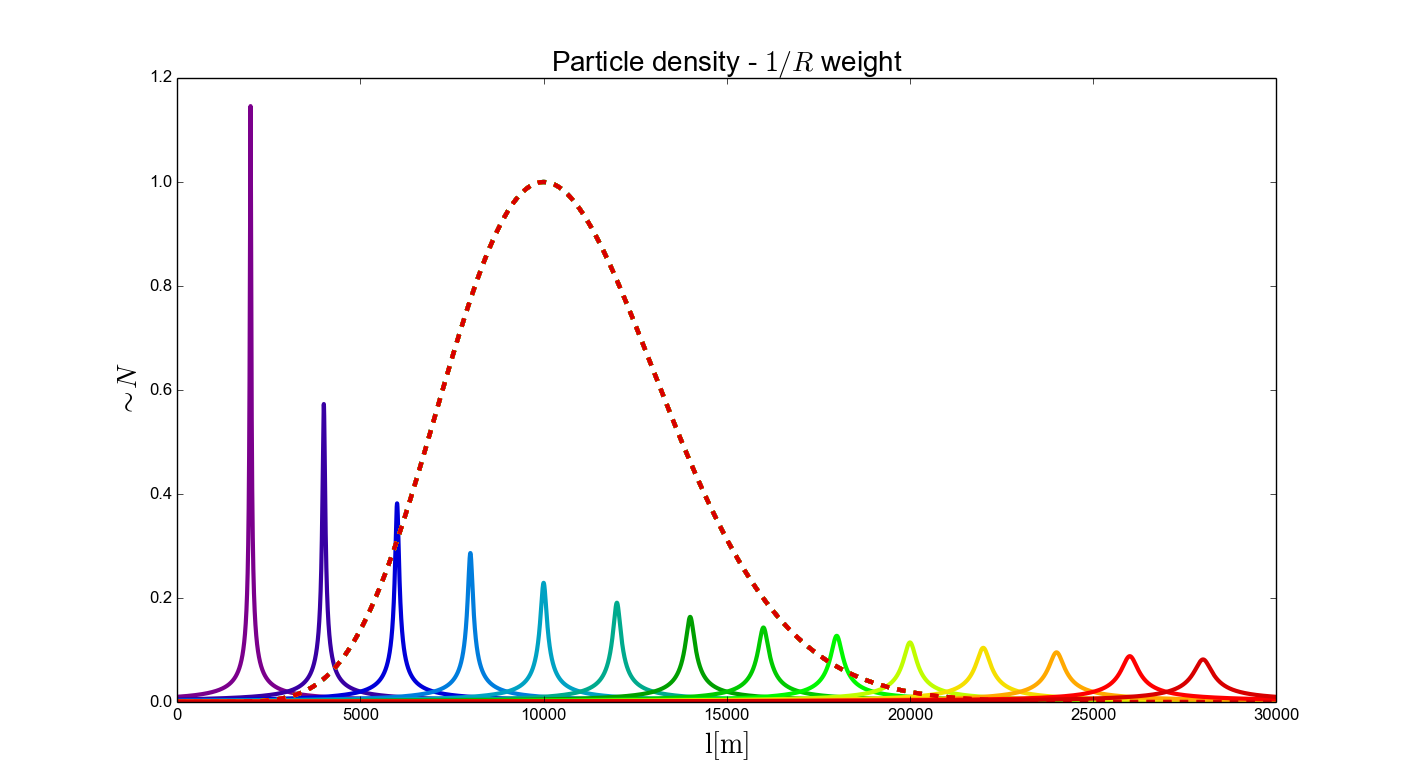
\includegraphics[width=0.8\textwidth]{./fig/EASRadio/timeDelay_pd}
		\caption{\label{fig:timeDelay_pd}
		En linea punteada se muestra la distribuci\'on de part\'iculas a lo largo del eje de la lluvia. En linea llena se grafica el factor $1/R$ para antenas en diferentes posiciones.
		El campo el\'ectrico registrado en cada antena ser\'a proporcional al producto de estas funciones.
		}
	\end{figure}
	A la hora de sumar las señales en cada bin temporal se utilizará el producto de ambas curbas para cada antena.
	
	Con los pesos calculados es posible integrar sobre la variable $t$ las curvas de la figura \ref{fig:timeDelay_at}, como en la ecuación \ref{eq:tint}.
	\begin{equation}
	S(t_i)=\sum_{l_i}w_i\Delta l_i
	\label{eq:tint}
	\end{equation}
	En esta, $S(t_i)$ es la señal recibida en $t_i\leq t<t_{i+1}$, $l_i$ son los $l_i:t_i\leq t(l_i)<t_{i+1}$, $w_i$ es su peso y $\Delta l_i$ es el ancho del paso elegido en $l$.
	El resultado de esta integral se expone en la figura \ref{fig:timeDelay_as} para diferentes valores de $d_a$.
	\begin{figure}[ht!]
		\centering
		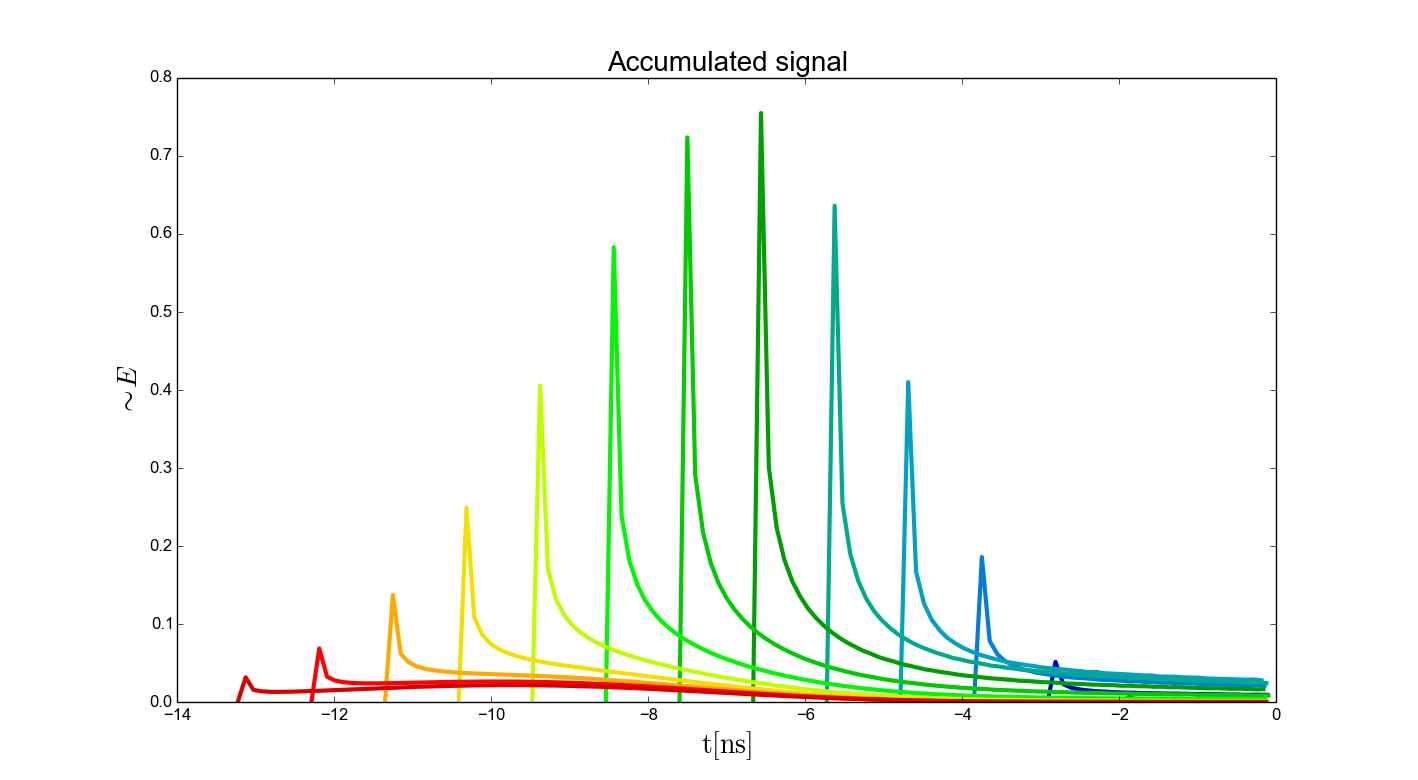
\includegraphics[width=0.8\textwidth]{./fig/EASRadio/timeDelay_as}
		\caption{\label{fig:timeDelay_as}
		Se\~nal acumulada en funci\'on del tiempo obtenida a partir de la ecuación \ref{eq:tint}.
		}
	\end{figure}
	Si bien el adelanto de la señal respecto de la referencia es de alguna decena de $\rm ns$, cada antena se encuentra separada al rededor de \cant{2000}{m}, o \cant{6000}{ns} entre sí, por lo que se puede suponer que para este tipo de lluvias (ES) la señal a nivel del suelo se desplaza aproximadamente a la velocidad de la luz.
	Finalmente, la figura \ref{fig:timeDelay_spa} muestra como es la evolución del máximo de la señal como función de $d_a$.	
	\begin{figure}[ht!]
		\centering
		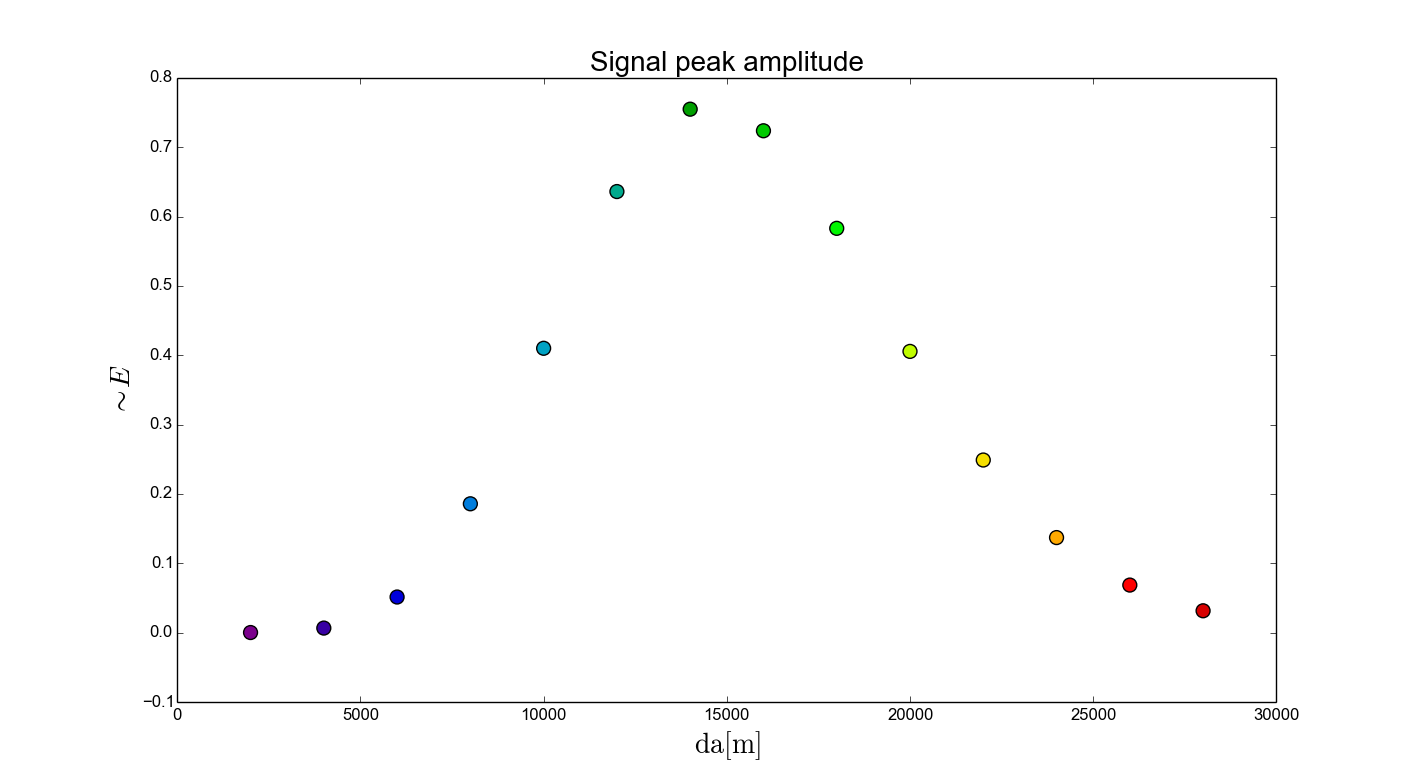
\includegraphics[width=0.8\textwidth]{./fig/EASRadio/timeDelay_spa}
		\caption{\label{fig:timeDelay_spa}
		M\'aximo de la se\~nal acumulada como función de la posici\'on de la antena.
		}
	\end{figure}
	La evolución del máximo de la señal presenta un máximo que se ubica en \cant{\sim 14000}{m}, que es la posición en la que se espera el máximo según lo expuesto en la sección \ref{sbsc:geom_emision} si se considera un cono \cher{} de \cant{1.4}{^\circ}.
	